\chapter{Experimental Results}

As presented in Chapter \ref{sec:sonar_section}, ultrasonic distance sensors can, at times, present challenging issues. Multipath and specular returns were encountered and lead to data like that shown in Figure \ref{fig:sonar4}. This data was taken while Nao walked down a straight hallway, with no other obstacles to occlude its path. The inconsistency of the data, at times, interferred with the Nao's ability to navigate it's environment. Despite these inconsistencies, the Nao was able to path plan various sorts of office-like environments.

\begin{figure}[H]
	\centering
	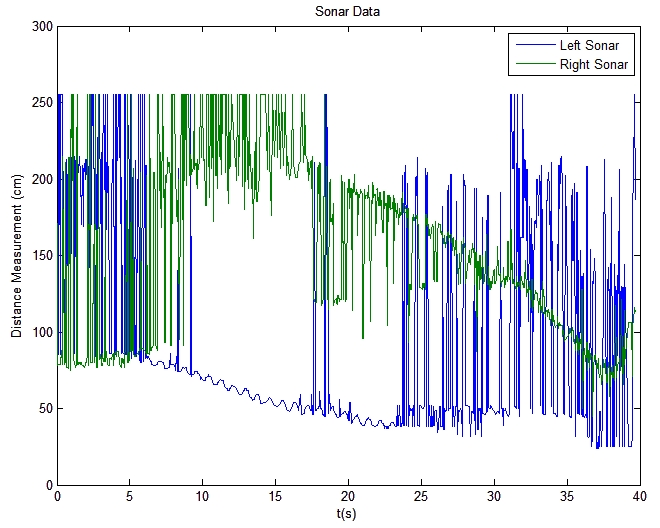
\includegraphics[width=\textwidth]{sonar4.jpg}
	\caption[Nao sonar data.]
	{Nao sonar data. The plot shows the distance data reported from the ultrasonic sensors while the Nao walked down a corridor.}
	\label{fig:sonar4}
\end{figure}
Figure \ref{fig:naoTime1} shows an experimental run of the Nao utilizing the GODZILA path planning algorithm. Nao was placed in a hallway setting with two cylindrical obstacles. The obstacles obstruct Nao's path to the goal, which was represented by a red cube measuring 10 cm x 10 cm x 8 cm. Nao is placed facing the goal. On start, Nao acquires the goal and walks towards it. Nao then guides around the first obstacle which sends it towards the second obstacle. Nao detects the second obstacle, guides around it, and walks to the goal.

\begin{figure}[h]
	\centering
	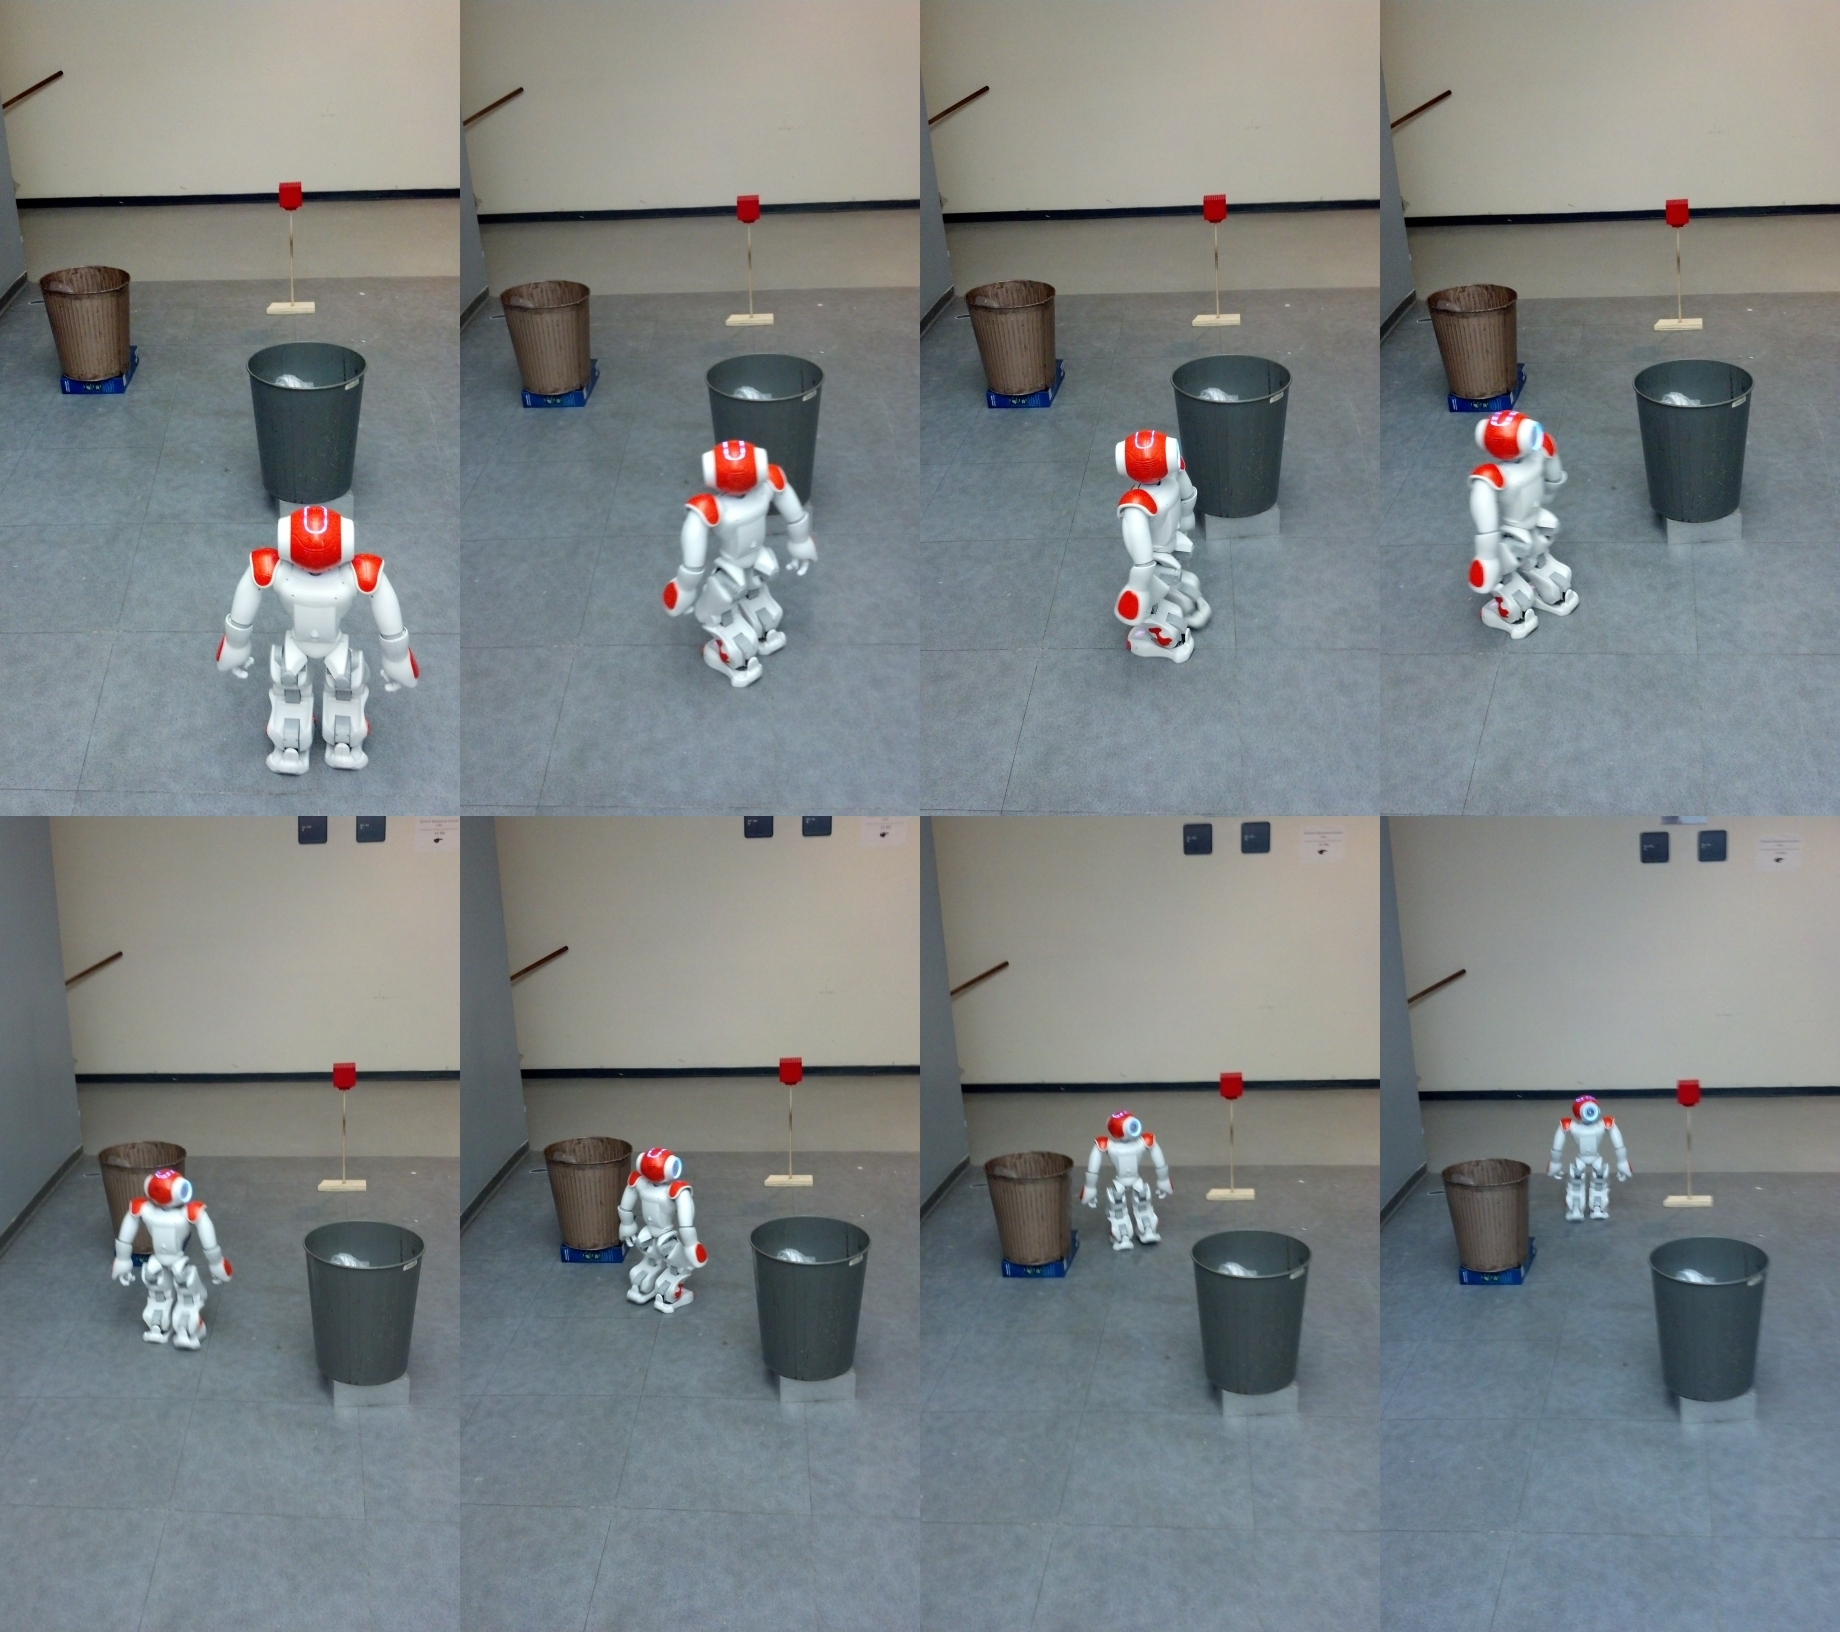
\includegraphics[width=\textwidth]{nao_time1.jpg}
	\caption[Nao time sequence.]
	{Nao time sequence. The Nao is started with the GODZILA path planning algorithm initiated. The goal location is indicated by the red cube. Two obstacles are obstructing the path to the goal. Nao sucessfully navigates around the obstacles to the goal.}
	\label{fig:naoTime1}
\end{figure}